
\chapter{Continuous probability distributions}

\section{Probability density function}

\dfn{Continuous random variable}{
    A random variable $X$ with $CDF F_X (x)$ is said to be continuous if $F_X (x)$ is a continuous function for all $x \in \mathbb{R}$.
}

Contrary to discrete random variables, the CDF of a continuous random variable is a continuous function (from both the left and right). For continuous random variables $P(X \le a) = P(X < a)$. 

$$P(X = x) = P(X \le x) - P(X < a)$$
$$= F_X (x) - \lim_{y \rightarrow X^-} F_X (y)$$
$$= F_X (x) - F_X (x)$$
$$= 0$$

Hence, single points have probability zero. Therefore:
$$P(X \le a) = P(X < a)$$

Since $F_X (x)$ is continuous for a continuous random variable $X$, we have:
$$P(x_1 \le X \le x_2) = P(x_1 \le X < x_2)$$
$$=P(x_1 < X \le x_2)$$
$$=P(x_1 < X < x_2)$$

\dfn{Probability density function}{
    Let $X$ be a continuous random variable with CDF $F_X (x)$. Then the function $f(x)$ is called a \textbf{probability density function (PDF)} of $X$ if:

    $$F_X (x) = \int_{-\infty}^{x} f_{X} (y) \,dx$$
}

\textbf{Properties of PDF $f_X (x)$}
\begin{enumerate}
    \item $f_X (x) \ge 0$ for $\forall{x} (- \infty < x < \infty)$
    \item $\int_{-\infty}^{\infty} f_X (x) \,dx = 1$
    \item We can obtain the CDF from a PDF and PDF from a CDF.
    \item By the definition of a PDF, $F_X (x) = \int_{-\infty}^{x} f_X (y) dy$. By the Fundamental Theorem of Calculus,
    $$F'_X(x) = \frac{d}{dx} \int_{-\infty}^{x} f_X (y) dy$$
    $$ = f_X (x)$$
\end{enumerate}

Any non-negative function can be used as a PDF. Suppose we have a function $g$ which satisfies property 1 of a PDF, but:
$$\int_{-\infty}^{\infty} g(x) dx = C \not = 1$$

We can normalize $g$ to get a PDF as follows:
$$f(x) = \frac{g(x)}{C}$$
where
$$\int_{-\infty}^{\infty} f(x) dx = \int_{-\infty}^{\infty} \frac{g(X)}{C} dx = 1$$

\ex{}{
    Given $f(y) = cy^2, 0 \le y \le 2$, and $f(y) = 0$ elsewhere, find the value of $c$ for which $f(y)$ is a valid density function.
}

\sol{}{
    For $f(y)$ to be a valid density function, we need $\int_{-\infty}^{\infty} f(y) dy = 1$ and $f(y) \ge 0$. 

    $f(y) \ge 0$ as long as $c \ge 0$. Now we need to normalize such that:
    $$\int_{-\infty}^{\infty} f(y) dy = 1$$
    $$\int_{-\infty}^{\infty} cy^2 dy = 1$$
    $$\implies \int_{-\infty}^{0} f(y) dy + \int_{-\infty}^{2} f(y) dy + \int_{2}^{\infty} f(y) dy = 1$$
    $$\implies \int_{-\infty}^{0} 0 dy + \infty{0}^{2} cy^2 dy + \infty{2}^{\infty} 0 dy = 1$$
    $$\implies \int_{0}^{2} cy^2 dy = 1$$
    $$c | \left[ \frac{y^3}{3} \right]_{0}^{2} |$$
    $$c (\frac{8}{3}) = 1$$
    $$c = \frac{3}{8}$$
}

\textbf{Comparing PDF and PMF}\\
Recall that the probability mass function is $P(X = x)$ and the probability density function is $f_X (x)$. The PMF gives single point probabibilities. The PDF does not give probabilities and can be greater than 1. However, when the PDF is integrated over a single interval, it could give a probability (that $X$ lies in a certain interval).\\

\textbf{Interpretation of PDF}\\
$$F'_X (x) = \frac{d}{dx} \int_{-\infty}^{X} f_X (y) dy = f_X (x)$$
$$F'_X (x) = \lim_{\Delta x\to 0} \frac{F_X (x + \Delta x) - F_X (x)}{\Delta x}$$
$$\approx \lim_{\Delta x \to 0} \frac{Pr(X \le x + \Delta x) - P(X \le x)}{\Delta x}$$
$$f_X (x) \approx \lim_{\Delta x \to 0} \frac{Pr (X \le x + \Delta x) - P(X \le x)}{\Delta x}$$
$$f_X(x) \approx Pr (X \le x _ \Delta x) - P(X \le x)$$ where $\Delta x \rightarrow 0$

This is the area under the curve for $(x \le X \le x + \Delta x)$, that is $\int_{x}^{x + \Delta x} f_X (y) dy$.

\section{Expected value and variance of a continuous random variable}
The expected value or mean of a continuous random variable $X$ is (where $f(x)$ is the PDF):
$$E(X) = \int_{-\infty}^{+\infty} xf(x) dx$$

The expected value of a random variable exists if $E(|X|) < \infty$.

The variance of a continuous random variable $X$ is:
$$E(X - \mu)^2 = \int_{-\infty}^{+\infty} (x- \mu)^2 f(x) dx$$
or
$$Var(X) = E(X^2) - [E(X)]^2$$
$$= \int_{-\infty}^{\infty} x^2 f(x) dx - [E(X)]^2$$

The $k^{th}$ moment of a continuous random variable $X$ is:
$$E(X^k) = \int_{-\infty}^{+\infty} x^k f(x) dx$$

The $k^{th}$ moment about the mean is:
$$E(X - \mu)^2 = \int_{-\infty}^{\infty}  (x - \mu)^2 f(x) dx$$

\ex{}{
    Suppose $X$ is a continuous random variable with the following probability function:
    \begin{equation}
    f(x) = 
        \begin{cases}
            3x^2 \text{ if } 0 < x < 1\\
            0 \text{ otherwise }
        \end{cases}
    \end{equation}

    Find $E(X)$ and $Var(X)$.
}

\sol{}{
    $$E(X) = \int_{-\infty}^{\infty} x f(x) dx$$
    $$= \int_{-\infty}^{0} x f(x) dx + \int_{0}^{1} x f(x) dx + \int_{1}^{\infty} x f(x) dx$$
    $$ = 0 + \int_{0}^{1} x \cdot 3x^2 dx + 0$$
    $$ = \infty_{0}^{1} 3x^3 dx$$
    $$= \left[ \frac{3x^4}{4} \right]_{0}^{1}$$
    $$=\frac{3}{4}$$
    Variance:
    $$Var(X) = E(X^2) - [E(X)]^2$$
    $$E(X^2) = \int_{-\infty}^{+\infty} x^2 f(x) dx$$
    $$=\int_{-\infty}^{0} 0 f(x) + \int_{0}^{1} x^2 (3x^2) dx + \int_{1}^{+\infty} 0 f(x) dx$$
    $$= 0 + \frac{3}{5} + 0$$
    $$= \frac{3}{5}$$
    $$Var(X) = E(X^2) - [E(X)]^2$$
    $$=\frac{3}{5} - (\frac{3}{4})^2$$
    $$=\frac{3}{80}$$
}


\section{Continuous probability distributions}

\subsection{Continuous uniform distribution}
\dfn{Continuous uniform distribution}{
    A continuous random variable $X$ is said to have a uniform distribution over the interval $[a,b]$, shown as $X \sim Uniform(a,b)$ if its PDF is given by:
    \begin{equation}
        f_X (x) = 
        \begin{cases}
            \frac{1}{b-a} & \text{ if } a < x < b\\
            0 & a < x \text{ or } b > x
        \end{cases}
    \end{equation}
}

\begin{figure}[H]
\centering
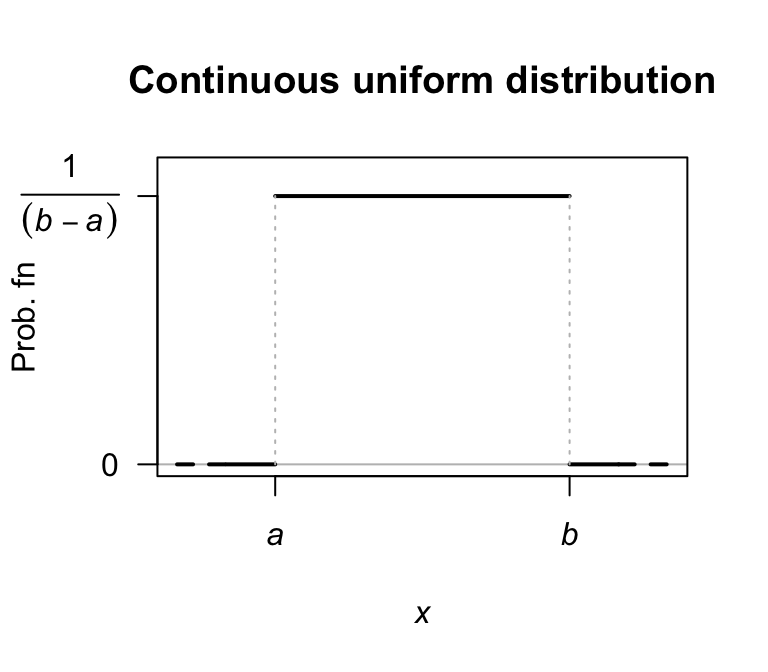
\includegraphics[width=0.45\textwidth]{images/cont_uniform_dist.png}
\caption{A uniform probability distribution}
\label{fig:sample}
\end{figure}

The \textbf{support} of continuous random variables is the set of all numbers whose probability density is strictly positive. Therefore the support of $X \sim Uniform(a,b)$ is $(a,b)$. The continuous distribution with $a = 0$ and $b = 1$ is called the standard uniform distribution. Observe that the probability of $X$ occuring between $a$ and $b$ is 1.

The \textbf{mean} of a continuous uniform random variable defined over the support $a < x < b$ is:
$$E(X) = \frac{a+b}{2}$$

\pf{Proof}{
    $$E(X) = \int_{a}^{n} x \frac{1}{b-a} dx$$
    $$= \frac{1}{b-a} | \frac{x^2}{2} |_{a}^{b}$$
    $$= \frac{b+a}{2}$$
}

The variance of a continuous uniform random variable defined over support is:
$$Var(X) = \frac{(b-a)^2}{12}$$

Proof using $Var(X) = E(X^2) - [E(X)]^2$.\\

\textbf{CDF} of a uniform random variable\\

We are looking for $P(X \le x)$. That is:
$$P(X \le x) = \int_{-\infty}^{x} f_X (x) dx$$
$$= \int_{a}^{x} \frac{1}{b-a} dy$$
$$=\frac{1}{b-a} \int_{a}^{x} 1 dy$$
$$= \frac{1}{b-a} | y |_{a}^{x}$$
$$=\frac{x-a}{b-a}$$

So define CDF as:
\begin{equation}
    F_X (x) = 
    \begin{cases}
        0 & x \le a\\
        \frac{x-a}{b-a} & a < x < b\\
        1 & x \ge b
    \end{cases}
\end{equation}

\begin{figure}[H]
\centering
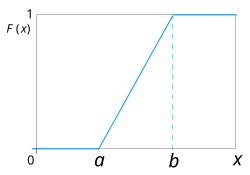
\includegraphics[width=0.45\textwidth]{images/cont_uniform_dist_cdf.png}
\caption{CDF of uniform probability distribution}
\label{fig:sample}
\end{figure}

\subsection{Gamma distribution}
\dfn{Gamma function}{
    The gamma function is defind as: $$\Gamma (\alpha) = \int_{0}^{\infty} x^{\alpha - 1} e^{-x} dx$$
}

We can often integrate by parts.

$$
\int x e^{-x} \, dx
$$
$$
u = x, \quad dv = e^{-x} \, dx
$$
$$
du = dx, \quad v = -e^{-x}
$$
$$
\int x e^{-x} \, dx = -x e^{-x} - \int (-e^{-x}) \, dx
$$
$$
= -x e^{-x} + \int e^{-x} \, dx
$$
$$
= -x e^{-x} - e^{-x} + C
$$
$$
= -e^{-x}(x + 1) + C
$$


Some important properties of $\Gamma (\alpha)$:
\begin{enumerate}
    \item $\Gamma(\alpha) = (\alpha - 1) \times \Gamma(\alpha - 1)$
    \item If $n$ is a positive integer then $\Gamma (n) = (n-1)!$
    \item $\Gamma (1/2) = \sqrt{\pi}$
\end{enumerate}

\dfn{Probability density function of normal distribution}{
    A continuous random variable follows a gamma distribution with parameters $\alpha > 0$ and $\beta > 0$ if its probability density function is:
    \begin{equation}
        f_X (x) = 
        \begin{cases}
            \frac{1}{\Gamma (\alpha)} \frac{1}{\beta ^{\alpha}} x^{\alpha - 1} e^{-x / \beta} & \text{ if } x > 0\\
            0 & \text{ otherwise }
        \end{cases}
    \end{equation}
}


\begin{figure}[H]
\centering
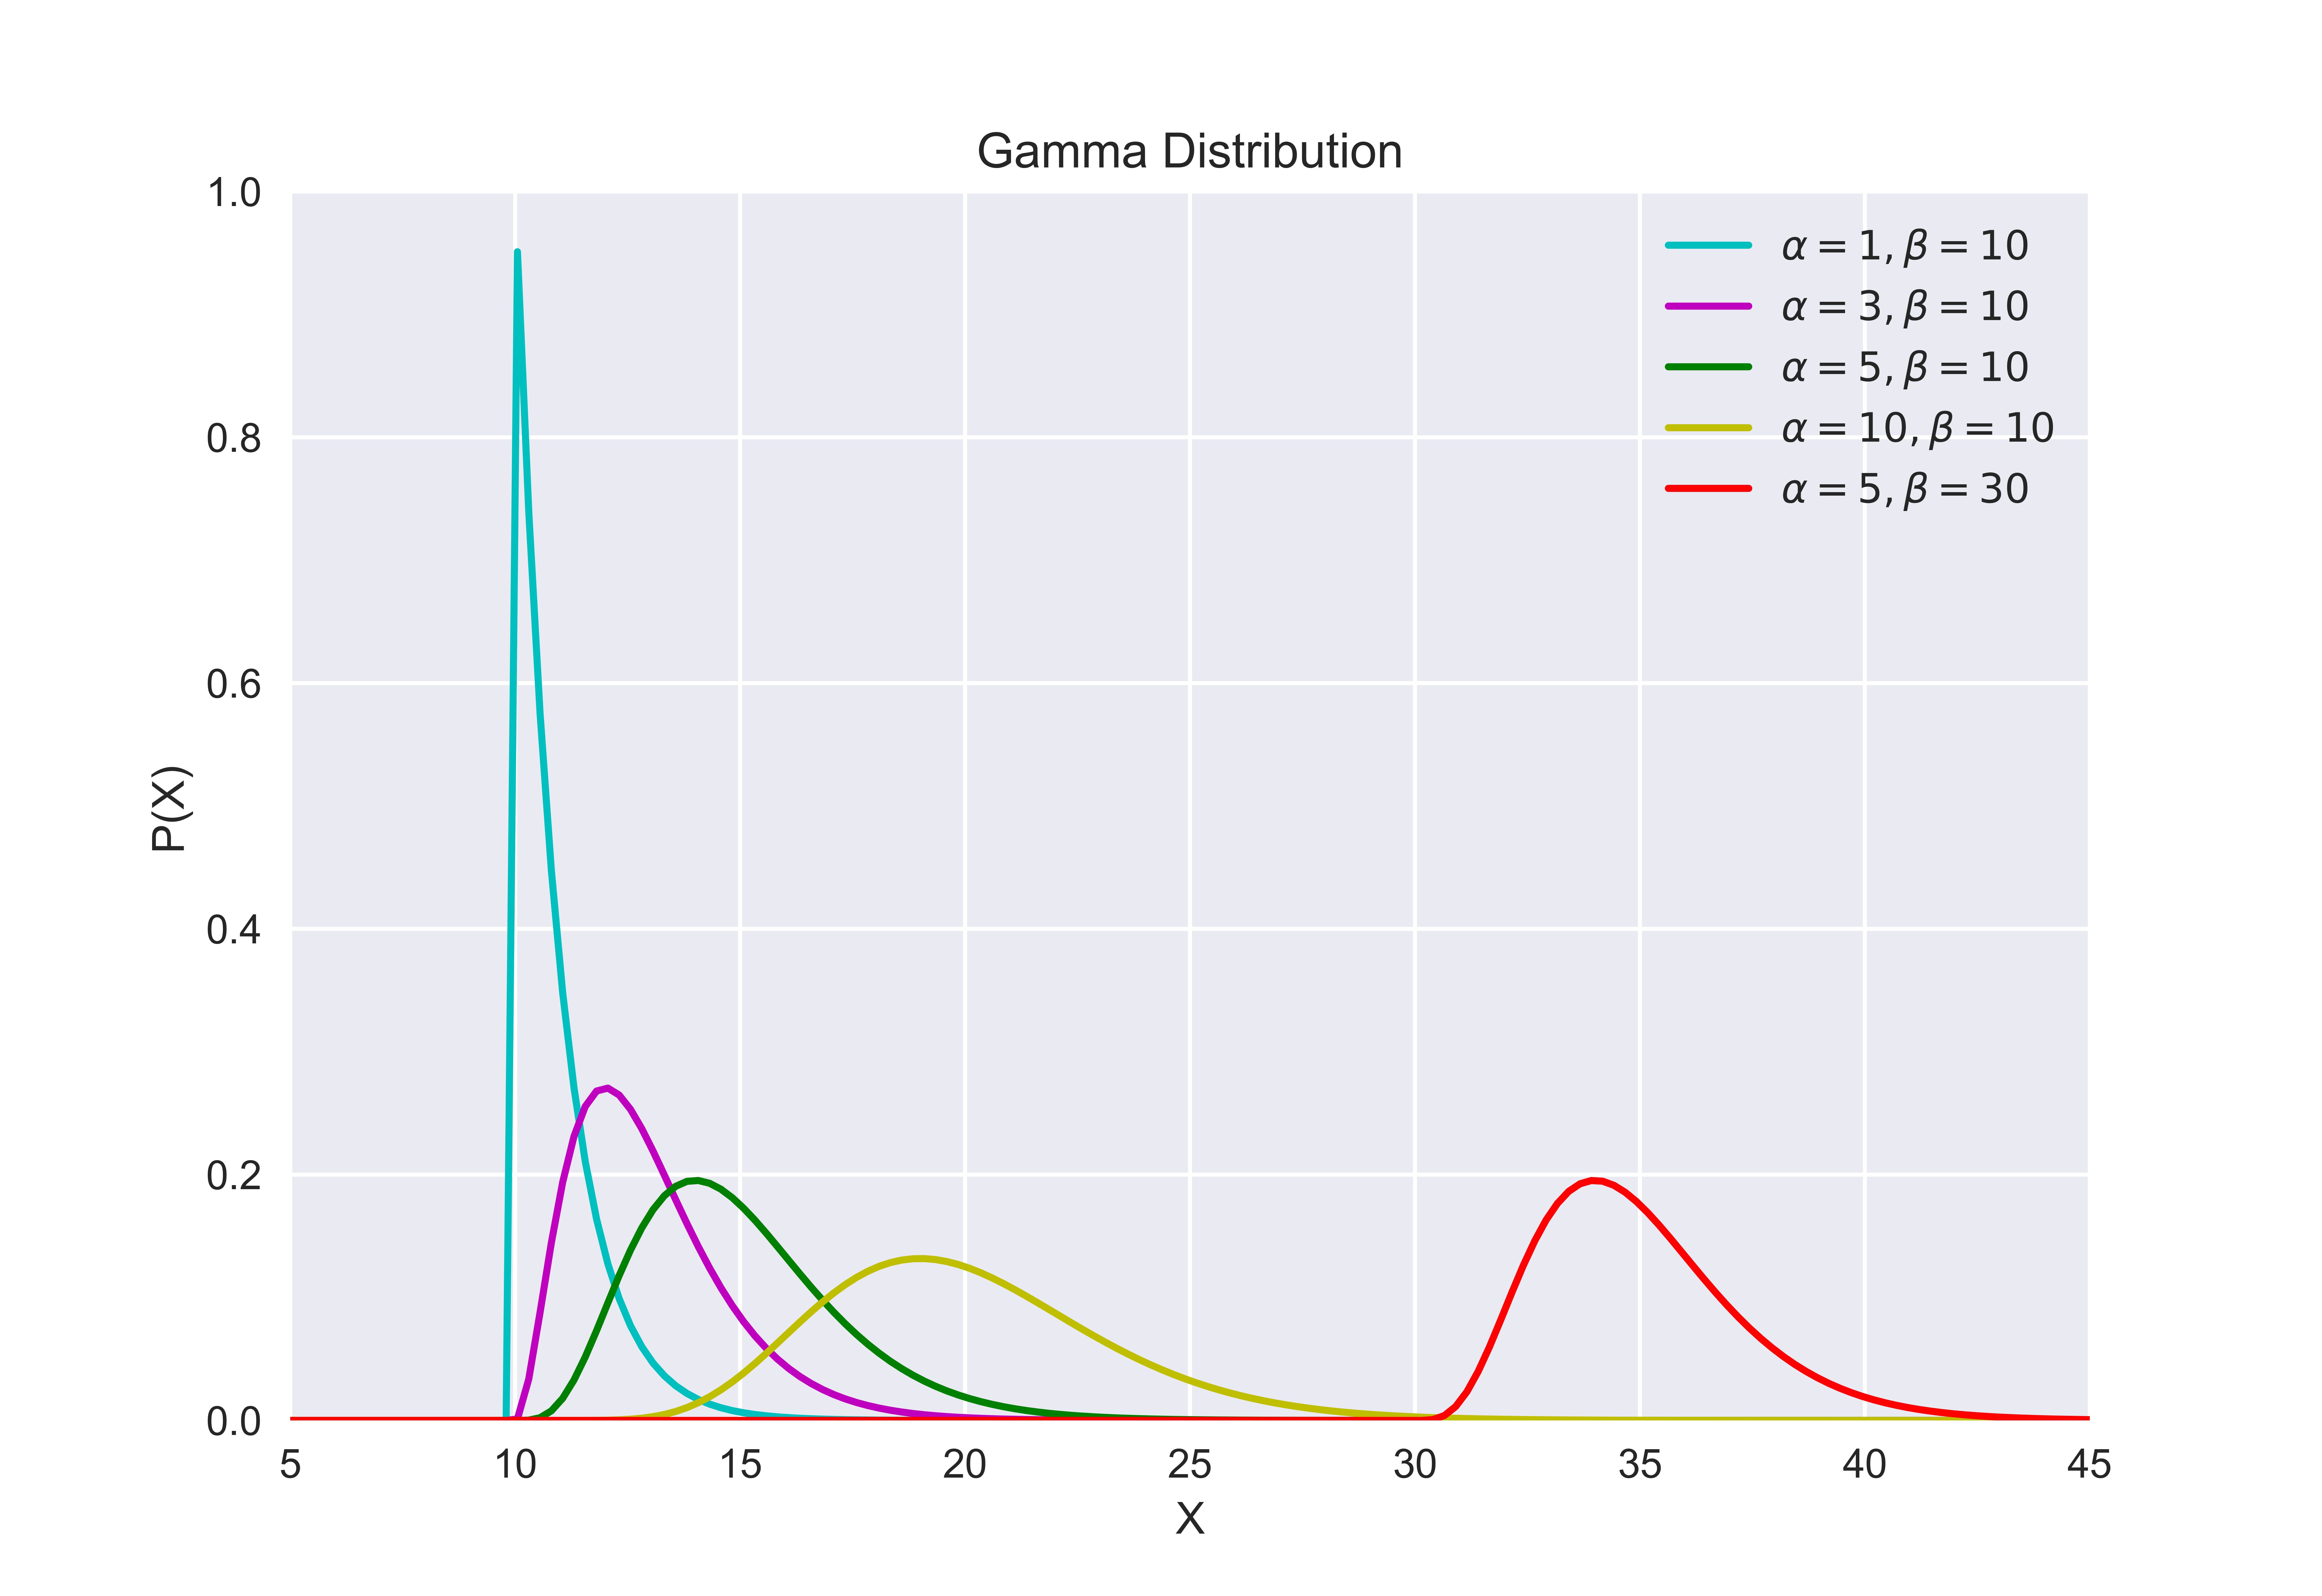
\includegraphics[width=1\textwidth]{images/gamma-dist.png}
\caption{CDF of uniform probability distribution}
\label{fig:sample}
\end{figure}

Finding the mean of the gamma distribution:
$$E(X) = \int_{-\infty}^{\infty} x \cdot \frac{1}{\beta^{\alpha} \Gamma (\alpha)} x^{\alpha - 1} e^{-x/ \beta} dx$$
$$= \frac{1}{\beta ^\alpha \Gamma (\alpha) } \int_{0}^{\infty} x^{\alpha} e^{-x / \beta} dx$$

We want to bring it into the gamma function form. Let $\frac{x}{\beta} = y$, therefore $dx = \beta dy$.
$$= \frac{1}{\beta ^\alpha \Gamma (\alpha) } \int_{0}^{\infty} (\beta y)^{\alpha} e^{-y} \beta dy$$
$$= \frac{\beta}{\Gamma (\alpha) } \int_{0}^{\infty} y^{\alpha} e^{-y} dy$$

Using recursive property of gamma function, where $\Gamma (\alpha + 1) = \int_{0}^{\infty} x^{\alpha} e^{-x} dx$, and $\Gamma (\alpha + 1) = \Gamma(\alpha) \cdot \alpha $.

$$ = \frac{\beta}{\Gamma (\alpha)} \Gamma (\alpha + 1) $$
$$= \frac{\beta \alpha \cdot \Gamma (\alpha)}{\Gamma \alpha}$$
$$= \beta \alpha$$

\textbf{Variance of the Gamma random variable}\\
We must first find $E(X^2)$. Use:
$$E(X^2) = \int_{0}^{\infty} x^2 f(x) dx$$
$$= \int_{0}^{\infty} \frac{1}{\Gamma (\alpha)} \frac{1}{\beta^{\alpha}} x^2 x^{\alpha - 1} e^{-x / \beta} dx$$
$$= \frac{1}{\Gamma (\alpha)} \frac{1}{\beta^{\alpha}} \int_{0}^{\infty} x^{\alpha + 1} e^{-x / \beta} dx$$

Let $x/ \beta = y \implies dx = \beta dy$. Therefore:
$$= \int_{0}^{\infty} x f(x) dx = \frac{1}{\Gamma (\alpha)} \frac{1}{\beta ^{\alpha}} \int_{0}^{\infty} (\beta y)^{\alpha + 1} e^{-y} \beta dy$$
$$= \int_{0}^{\infty} x f(x) dx = \frac{1}{\Gamma (\alpha)} \beta^2 \int_{0}^{\infty} y^{\alpha + 1} e^{-y} dy$$

From the recursive definition of $\Gamma(\alpha)$, where $\Gamma (\alpha + 2) = (\alpha + 1) \cdot \Gamma (\alpha + 1)$. Then $\Gamma (\alpha + 2) = (\alpha + 1) \cdot (\alpha) \Gamma (\alpha)$:

$$= \alpha (\alpha + 1) \beta ^2 \frac{1}{\Gamma (\alpha)} \Gamma (\alpha)$$
$$E(X^2) = \alpha (\alpha + 1) \beta ^2$$

Now subtracting $[E(X)]^2$ to find variance:
$$Var(X) = \alpha (\alpha + 1) \beta^2 - (\alpha \beta )^2$$
$$Var(X) = \beta^2(\alpha^2 + \alpha - \alpha^2) $$
$$Var(X) = \beta^2 \alpha$$

\ex{}{
    Show that 
    \begin{equation}
        f_X (x) = 
        \begin{cases}
            \frac{1}{\Gamma (\alpha)} \frac{1}{\beta ^{\alpha}} x^{\alpha - 1} e^{-x / \beta} & \text{ if } x > 0\\
            0 & \text{ otherwise }
        \end{cases}
    \end{equation}
    is a PDF. 
}

\sol{}{
    $f(x) > 0$ holds by definition. Now we must establish that $\int_{0}^{\infty} f(x) dx = 1$. 

$$= \frac{1}{\Gamma (\alpha) \beta ^ \alpha}\int_{0}^{\infty} x^{\alpha - 1} e^{-x / \beta} dx$$
Let $\frac{x}{\beta} = y$. Then $dx = \beta dy$. 
$$= \frac{1}{\Gamma (\alpha) \beta ^ \alpha}\int_{0}^{\infty} (\beta y)^{\alpha - 1} e^{-y} \beta dy$$
$$= \frac{1}{\Gamma (\alpha) \beta ^ \alpha} \beta^{\alpha - 1} \beta \int_{0}^{\infty} 
y^{\alpha - 1} e^{-y} dy$$
$$= \frac{1}{\Gamma (\alpha) \beta ^ \alpha} \beta^{\alpha} \int_{0}^{\infty} y^{\alpha - 1} e^{-y} dy$$
$$= \frac{1}{\Gamma (\alpha)}  \int_{0}^{\infty} y^{\alpha - 1} e^{-y} dy$$
$$= \frac{1}{\Gamma (\alpha)}  \Gamma(\alpha)$$
$$= 1$$
}



\textbf{CDF of the Gamma distribution}\\

Looking for $P(X \le x)$. 

$$P(X \le x) = \int_{0}^{x} f_X (x) dx = \int_{0}^{x} \frac{1}{\beta ^ \alpha \Gamma(\alpha)} x^{\alpha - 1} e^{-x / \beta} dx$$

This integral does not have a closed form. Will need to discuss as cases.

\subsection{Chi-square distribution}

\dfn{Probability density function of the chi-square distribution}{
    Let $X$ follow a gamma distribution with $\alpha = v / 2$ and $\beta = 2$, where $v$ is a positive integer. Then the probability density function of $X$ is:
    \begin{equation}
        f(x) = 
        \begin{cases}
            \frac{1}{\Gamma (v/2)} \frac{1}{2^{v/2}} x^{v/2-1} e^{-x/2} & \text{ if } x > 0\\
            0 & \text{otherwise}
        \end{cases}
    \end{equation}
}

\textbf{Properties of the Chi-square distribution}\\
Let $X \sim \chi ^2 (v)$
$$E(X) = \alpha \beta = v / 2 \times 2 = v$$
$$Var(X) = \alpha \beta ^2 = v /2 \times 2^2 = 2v$$
Will not discuss too much in this class. Used in hypothesis testing, not usually modelling.

\subsection{Exponential distribution}
Another special case of the gamma distribution, where the shape parameter $\alpha = 1$ and $\beta > 0$:

\begin{equation}
    f(x) = 
    \begin{cases}
        \frac{1}{\Gamma (\alpha)} \frac{1}{\beta ^ \alpha} \cdot x^{\alpha - 1} e^{-x / \beta} & \text{ if } x > 0\\
        0 & \text{ otherwise }
    \end{cases}
\end{equation}

Substituting in $\alpha = 1$:

\begin{equation}
    f(x) = 
    \begin{cases}
        \frac{1}{\beta} \cdot e^{-x / \beta} & \text{ if } x > 0\\
        0 & \text{ otherwise }
    \end{cases}
\end{equation}

\dfn{Probability density function of the normal distribution}{
\begin{equation}
    f(x) = 
    \begin{cases}
        \frac{1}{\beta} \cdot e^{-x / \beta} & \text{ if } x > 0\\
        0 & \text{ otherwise }
    \end{cases}
\end{equation}
}

\textbf{Properties of the exponential distribution}\\
Let $X \sim exp(\beta)$, then
\begin{enumerate}
    \item $E(X) = \beta$
    \item $Var(X) = \beta ^2$
    \item The probability of future events does not depend on which previous events occurred. That is, $P(X \ge a + x | P \ge a) = P(X \ge x)$.
\end{enumerate}

If $X \sim exp(\beta)$, then

While the gamma distribution has no closed form solution, the CDF of the exponential distribution does:

\begin{equation}
    F(x) = 
    \begin{cases}
        0 & \text{ for } x < 0\\
        \int_{0}^{x} \frac{1}{\beta} e^{-y / \beta} dy & \text{ if } x > 0
    \end{cases}
\end{equation}


And therefore:

$$\int_{0}^{x} \frac{1}{\beta} e^{-y / \beta} dy = 1 - e^{-x / \beta}$$

\nt{
    The exponential distribution is usually used to measure waiting times.
}

\ex{}{
    A manufacturing plant uses a specific bulk product. The amount of product used in one day can be modelled by an exponential distribution with $\beta = 4$ (measurement in tons). Find the probability that the plant will use more than 4 tons in a given day.
}

\sol{}{
    The amount of product used in one day is modelled as:
    $$X \sim exp(\beta)$$
    Then we have:
    $$E(X) = \beta = 4$$
    We are looking for $P(X > 4)$. We have the CDF:
    $$P(X > 4) = 1 - P(X \le 4)$$
    $$ = 1 - (1 - e^{-x / \beta})$$
    $$ = 1 - (1 - e^{-4 / 4})$$
    $$ = \frac{1}{e}$$
    Alternatively, you could integrate $\int_{4}^{\infty} \frac{1}{\beta} e^{-x / \beta} dx$.
}

\ex{}{
    Suppose the time you spend waiting for a job offer has an exponential distribution with a mean of 10 days. Suppose you have already spent 10 days waiting. What is the probability that you will spend at least an additional three days waiting for the offer?
}

\sol{}{
    We have that $E(X) = 10 = \beta$. Looking for:
    $$P(X > 10 + 3 | x > 10)$$
    $$ = \frac{P(X > 13 \cap X > 10)}{P(X > 10)}$$
    $$ = \frac{X > 13}{X > 10}$$
    $$ = \frac{1 - P(X \le 13)}{1 - P(X \le 10)}$$
    $$ = \frac{1 - (1 - e^{-13 / \beta})}{1 - (1  - e^{-10 / \beta})}$$
    $$= e^{-13 / \beta} \cdot e^{10 / \beta}$$
    $$ = e^{-3 / \beta}$$
    $$ = P (X > 3)$$

    Observe the memory-less property.
}

\subsection{Normal distribution}

\dfn{Probability density function of normal distribution}{
    $$f(x) = \frac{1}{\sqrt{2\pi} \sigma} e^{-(x - \sigma)^2 / 2 \sigma ^2}$$

    Where $\sigma = 0$ and $\sigma^2 = 1$ in the standard normal distribution.
}

\textbf{Properties of the normal distribution}\\
\begin{enumerate}
    \item The mean $\sigma$ locates the centre of the distribution.
    \item The shape of the distribution is determined by $\sigma$, which is the population standard deviation.
    \item Large values of $\sigma$ reduce the height of the curve and increase the spread; small values of $\sigma$ increase the height of the curve and reduce the spread.
    \item The normal distribution is perfectly symmetric about its mean $\sigma$.
    \item We have to know the numerical values of $\mu$ and $\sigma$ to graph the normal curve.
\end{enumerate}

\dfn{Standard normal distribution}{
    The normal distribution with $\mu = 0$ and $\sigma = 1$ is known as the standard normal distribution. To convert a normal random variable $X$ to a standard normal variable $Z$, we use:
    $$Z = \frac{X - \mu}{\sigma}$$
    Also have that:
    $$X = \mu + \sigma Z$$
}

\thm{}{
    If $X$ is normally distributed with mean $\mu$ and variance $\sigma ^2$, then:
    $$Z^2 = (\frac{X - \mu}{\sigma})^2$$
    is Chi-squared distributed with one degree of freedom.
}

\ex{}{
    Assume that for the American population the IQs are normally distributed with $\mu = 100$ and $\sigma = 10$. 
    \begin{enumerate}
        \item What is the probability that a randomly selected American has an IQ below 90?
        \item What is the probability that a randomly selected American has an IQ above 120?
        \item What is the IQ of a randomly chosen American if their IQ is more than the IQ of 80\% of the Americans.
    \end{enumerate}
}

\sol{}{
    We have that $X \sim (100, 10^2)$. Use standardization.
    \begin{enumerate}
        \item $P(X < 90) = P(X \le 90) = P(\frac{X - \mu}{\sigma} < \frac{90 - 100}{10} = P(Z < - 1)$
        By symmetry, have that:
        $$= P(Z > 1)$$
        $$=1 - P(Z \ge 1)$$
        $$ = 1 - 0.8413$$
        \item $P(X > 120) = 1 - P(X \le 120) $
        $$P(\frac{x - \sigma}{\mu} > \frac{120 - 100}{10}$$
        $$ = 1- P(Z \le 2)$$
        $$ = 1 - 0.9772$$
        \item $P(X < x) = 0.8$. So:
        $$= P(\frac{X - \mu}{\sigma} < \frac{z - \mu}{\sigma}) = 0.8$$
        $$ = P(Z < z) = 0.8$$
        Find that $z = 0.845$. Therefore:
        $$0.845 = \frac{x - 100}{10}$$
        $$ x = \mu + \sigma z$$
        $$x = 100 + 10(0.845)$$
        $$x = 108.45$$
    \end{enumerate}
}

\qs{}{
    Wires manufactured for use in a computer system are specified to have resistances between 0.12 and 0.14 ohms. The actual measured resistances of the wires produced by company A have normal distribution with mean 0.13 ohms and standard deviation 0.005 ohms.
    \begin{enumerate}
        \item What is the probability that a randomly selected wire from company A's production will meet specifications?
        \item If four of these wires are used in each computer system and all are selected from company A, what is the probability that all 4 in a randomly selected system will meet specifications?
    \end{enumerate}
}

\sol{}{
    \begin{enumerate}
        \item Looking for $P(0.12 < x < 0.14)$
        $$= P(X < 0.14) - P(x < 0.12)$$
        $$ = P(\frac{X - \mu}{\sigma} \le \frac{0.14 - 0.13}{0.005}) - (...)$$
        \item We have 4 trials with failure and success. We can model with a binomial distribution. $p$ is found in $a$.
        $$P(Y = 4) = \binom{4}{4} p^4 ( 1- p)^0$$
    \end{enumerate}
}

\qs{}{
    A soft-drink machine can be regulated so that it discharges an average of $\mu$ ounces per cup. If the ounces of fill are normally distributed with $\sigma = 0.3$, give the setting for $\mu$ so that 8-ounce cups will overflow only 1 \% of the time.
}

\sol{}{
    $P(X > 8) = 0.01$. So $P(\frac{x - \mu}{\sigma} > \frac{8 - \mu}{\sigma}) = 0.01$
    $$P(Z > z) = 0.01$$
    $$P(Z > z) = 1 - P(Z \le z)$$
    $$P ( Z \le z) = 0.99$$
    Looking for $z$ that corresponds. Then use $x = \mu + \sigma z$ to find $\mu$. 
}
